
\documentclass[conference]{IEEEtran}
\usepackage[encapsulated]{CJK}
\usepackage{cite}
\usepackage{amsmath,amssymb,amsfonts}
\usepackage{algorithmic}
\usepackage{graphicx}
\usepackage{tabularx}
\usepackage{booktabs}
\usepackage{color}
\begin{document}
\begin{CJK}{UTF8}{bsmi}
\title{Timing-Feedback Adaptive Scheduler for Split-6 Latency Reduction}
\author{
\author{\IEEEauthorblockN{
        Ming-Hong HSU\IEEEauthorrefmark{1}, 
        Ray-Guang Cheng\IEEEauthorrefmark{1},
        Co-author 1\IEEEauthorrefmark{2}
        \\
  }
 \IEEEauthorblockA{\IEEEauthorrefmark{1}
Dept. of Electronic and Computer Engineering, National Taiwan University of Science and Technology, Taiwan
  }
  Email: crg@mail.ntust.edu.tw
}

\IEEEauthorblockA{
Department of Electronic and Computer Engineering, National Taiwan University of Science and Technology\\
Taipei, Taiwan, Republic of China \\
Email: crg@mail.ntust.edu.tw}
}

\maketitle
% 1. 請先各自複製本範本的內容，根據這裡所點出的大綱來寫，無關的內容請勿放入。自己加的內容請用「藍字」，老師改過需要確認會用「紅字」，紅字內容確認無誤的字句請自行改為黑字，有問題改成「藍色」。
% 2. 縮寫字第一次出現前記得要先定義，原則上只有句首第一個字母大寫，請勿誤用！
% 3. 請用國中英文直述句來寫，正確性最重要
% 4. 本範本請先寫System Model、Propose Solution, 以及 Numercial/Experimental Results。Introduction請留到最後
% 5. Introduction僅留下「絕對必要」資訊(沒提到後面就講不下去)即可！
% 6. 使用任何變數前請先「定義」，寫下變數與公式前，請先想清楚，這是「問題」(I/P)、「答案」(O/P)、「推導過程」(Your Algorithm)、還是「範例」(Example)
% 問題與答案放在System Model，
% 推導過程放在Analytical Model，
% 範例放在Numercial Results

Abstract Section (before Introduction)
Add a clear placeholder for an abstract:

Purpose: Briefly summarize the problem, method, results, and contribution.

Word count: typically 150–250 words.

Keywords: list 3–6 keywords.

\section{Introduction}
{\color{blue}
Directly reusing the FAPI slot.indication mechanism in nFAPI mode without following the SCF specification leads to significant latency because FAPI timing control was not designed for nFAPI’s transport and synchronization characteristics. Automated testing and analysis are required to detect and verify the timing delays caused by non-compliant implementations with the SCF specification.

Each step of the nFAPI procedure must be individually measured and analyzed to isolate delay sources through repeated end-to-end testing. Continuous automated testing, data collection, and graphical analysis are needed to compare delay patterns and identify timing bottlenecks efficiently.
}

\subsection{Related Works}
{\bf Purpose:} To show how your work fits into the existing body of knowledge, and how it differs from or improves upon previous work.

Typical content:
\begin{itemize}
\item Summary of key prior research
\item Strengths and limitations of existing approaches
\item Comparison to your approach
\item Justification for why a new approach is needed
\end{itemize}

Example phrases:
\begin{itemize}
\item “Several studies have explored …”
\item “Unlike [Author], we propose …”
\item “Prior work has not considered …”
\end{itemize}

% Background Knowledge directly related to Your Thesis Title

% Related Work

% Contribution: The last TWO paragraphs of your paper.
The main contributions of this paper are summarized as follows.
\begin{itemize}
\item A fully SCF-compliant nFAPI implementation flow is established, replacing the legacy slot.indication mechanism with a delay-management process and introducing a VNF-side timing-window maintenance algorithm to cover undefined timing logic in the standard.
\item An SMO RAPP module is developed to automate end-to-end testing, data acquisition, and chart generation, enabling validation and optimization of the proposed delay-management mechanism.
\end{itemize}

The rest of the paper is organized as follows. Section II defines the system model/architecture considered in this paper. The proposed analytical model/method is given in Section III. Section IV shows the numerical results. Concluding remarks are given in Section VI.


\section{System Model}
\label{sec:system_model}

{\color{blue}
Figure~\ref{fig:system_model} illustrates the system architecture of the proposed Timing-Feedback Adaptive Scheduler within a Split-6 RAN environment. The system comprises two main entities: the Virtual Network Function (VNF) and the Physical Network Function (PNF), connected via a packet-switched network.

The VNF hosts the upper layer protocol stack and the scheduler. To minimize transmission latency and ensure synchronization with the PNF, the VNF implements a feedback-based timing mechanism. The key components include:

\begin{itemize}
    \item \textbf{Timing-Feedback Adaptive Module}: This module acts as the core controller. It receives timing feedback from the PNF, specifically the difference between the packet arrival time and the expected slot time (denoted as late by $N$ $\mu$s or early by $M$ $\mu$s). It also incorporates internal scheduler timing metrics. Based on these inputs, it dynamically computes the optimal sleep duration for the VNF timing thread to align with the PNF's slot cycle.
    \item \textbf{VNF Timing Thread}: This thread is responsible for triggering the scheduler instances. It utilizes the corrected timing provided by the Adaptive Module to wake up at the precise moment, compensating for network jitter and processing delays.
    \item \textbf{Scheduler}: Detailed scheduling operations are performed here. Multiple scheduler instances generate the Transmission Time Interval (TTI) messages, which are then transmitted to the PNF.
    \item \textbf{PNF}: The Physical Network Function receives the TTI messages for radio transmission. It measures the arrival time of these messages and feeds this "Timing Info" back to the VNF, closing the control loop. The specific parameters included in the Timing Info message are summarized in Table~\ref{tab:timing_info}, as defined in the 5G nFAPI Specification~\cite{nfapi_spec}.
\end{itemize}
}

\begin{table}[htbp]
\caption{nFAPI Timing Info Parameters~\cite{nfapi_spec}}
\label{tab:timing_info}
\begin{center}
\begin{tabularx}{\columnwidth}{l|l|X}
\toprule
\textbf{Field} & \textbf{Type} & \textbf{Description} \\ \midrule
Last SFN / Slot & uint16\_t & The completed SFN (0--1023) and slot (0--159) that triggered the message. \\ 
Time Since Last Info & uint32\_t & Time in ms since the last Timing Info message was sent. \\ 
Jitter & uint32\_t & Inter-message jitter ($\mu$s) for DL\_TTI, TxData, UL\_TTI, and UL\_DCI. \\ 
Latest Delay & int32\_t & Latest delay offset ($\mu$s) from acceptable window. Positive: late, negative: early. \\ 
Earliest Arrival & int32\_t & Earliest arrival offset ($\mu$s) from acceptable window. \\ 
Subcarrier Spacing & uint8\_t & SCS index (0: 15kHz to 4: 240kHz) as defined in TS38.211. \\ \bottomrule
\end{tabularx}
\end{center}
\end{table}

\begin{table}[htbp]
\caption{nFAPI Delay Management Timing Offset Parameters~\cite{nfapi_spec}}
\label{tab:delay_mgmt_offsets}
\begin{center}
\begin{tabularx}{\columnwidth}{X|l|X}
\toprule
\textbf{Parameter} & \textbf{Type} & \textbf{Description} \\ \midrule
Timing offsets (DL\_TTI, UL\_TTI, UL\_DCI, Tx\_Data) & uint32\_t & The timing offset ($\mu$s) before the slot start that the corresponding request must be received at PHY. \\ \bottomrule
\end{tabularx}
\end{center}
\end{table}

\begin{table}[htbp]
\caption{nFAPI Delay Management Configuration Parameters}
\label{tab:delay_mgmt_config}
\begin{center}
\begin{tabularx}{\columnwidth}{l|p{1.5cm}|X}
\toprule
\textbf{Parameter} & \textbf{Type} & \textbf{Description} \\ \midrule
timingWindow & uint16\_t & Timing window for delay management. See section 3.2.9 of [10] \\
timingMode & uint8\_t & Timing mode for Timing Info. See section 3.2.9 of [10] \\
timingPeriod & uint8\_t & Timing period for Timing Info. See section 3.2.9 of [10] \\ \bottomrule
\end{tabularx}
\end{center}
\end{table}

{\color{blue}
The primary objective of this system is to adaptively adjust the VNF's execution offset such that TTI messages arrive at the PNF within the valid reception window, thereby avoiding slot drops due to late arrival while minimizing buffering latency caused by excessive earliness.

\begin{figure}[htbp]
  \centerline{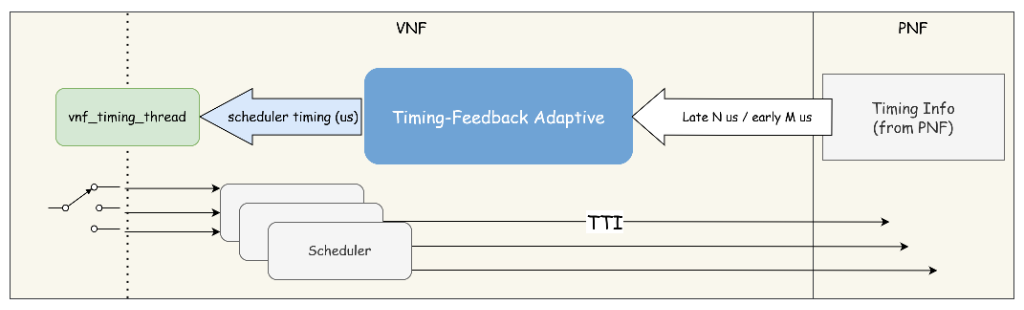
\includegraphics[width=1\columnwidth]{figures/system_model.png}}
  \caption{System Model of the Timing-Feedback Adaptive Scheduler.}
  \label{fig:system_model}
\end{figure}
}


\section{Proposed Method}
\label{sec:proposed_method}

{\color{blue}
To address the timing synchronization challenges in Split-6 RAN, we propose a Timing-Feedback Adaptive Scheduler. This mechanism introduces a closed-loop control system that dynamically adjusts the VNF's execution timing based on feedback from the PNF. As shown in Section \ref{sec:system_model}, the core objective is to minimize the timing difference between the arrival of TTI messages and the PNF's slot boundary, ensuring reliable transmission while minimizing latency. The proposed method consists of three key components: Jitter Mitigation via Baseline Envelope, Drift Prevention with a Time Bank mechanism, and Severe Deviation Handling.

\subsection{Dynamic Timing Adjustment Algorithm}
The core of the proposed method is an adaptive algorithm that calculates the optimal sleep duration ($T_{sleep}$) for the VNF timing thread.
Let $t_{arrival}$ be the arrival time of the TTI message at the PNF and $t_{slot}$ be the start time of the corresponding slot. The timing error $\Delta t$ is defined as:
}

\subsection{VNF-PNF Clock Synchronization}
{\color{blue}
To achieve precise time alignment between the VNF and PNF, a four-way handshake mechanism (Node Sync) is employed. Let $t_1$ be the timestamp when the VNF sends a synchronization request, $t_2$ and $t_3$ be the timestamps when the PNF receives and responds to the request, and $t_4$ be the timestamp when the VNF receives the response. The clock offset $\Delta t_{offset}$ and the one-way delay $T_{owd}$ are calculated as follows:
}
\begin{equation}
    \Delta t_{offset} = \frac{(t_2 - t_1) - (t_4 - t_3)}{2}
\end{equation}
\begin{equation}
    T_{owd} = \frac{(t_4 - t_1) - (t_3 - t_2)}{2}
\end{equation}
{\color{blue}
A positive $\Delta t_{offset}$ indicates that the VNF clock is lagging behind the PNF, while a negative value indicates it is ahead. To maintain a stable buffer at the PNF, a target margin $T_{margin}$ is added to the adjustment. The resulting slot-level adjustment $N_{slot\_adj}$ and microsecond-level adjustment $T_{us\_adj}$ are:
}
\begin{equation}
    N_{slot\_adj} = \lfloor \frac{\Delta t_{offset} + T_{margin}}{T_{slot}} \rfloor
\end{equation}
\begin{equation}
    T_{us\_adj} = (\Delta t_{offset} + T_{margin}) \pmod{T_{slot}}
\end{equation}

{\color{blue}
\subsection{Jitter Mitigation via Baseline Envelope}
Network jitter and processing variations can cause significant fluctuations in $\Delta t$. Direct reaction to every instantaneous value would lead to system instability. To mitigate this, we employ a Baseline Envelope mechanism.
The system maintains a variable $E_{base}$ representing the minimum observed processing and transmission delay.
\begin{itemize}
    \item \textbf{Fast Attack}: If the current measured delay $d_{curr}$ is less than $E_{base}$, we update $E_{base} = d_{curr}$. This allows the system to quickly adapt to improved network conditions.
    \item \textbf{Slow Decay}: If $d_{curr} > E_{base}$, we treat the excess as potential jitter. $E_{base}$ is slowly incremented (decayed) over time to ensure it doesn't get stuck at a transient minimum.
\end{itemize}
This envelope provides a stable reference point, effectively filtering out high-frequency noise.

\subsection{Drift Prevention with Time Bank Mechanism}
Traditional Proportional-Integral (PI) controllers can suffer from integral windup or oscillation in this context. We propose a "Time Bank" mechanism, utilizing a variable $T_{pending}$, to manage accumulated timing deviation without over-correction.
\begin{itemize}
    \item \textbf{Accumulation}: When the system is late ($\Delta t > 0$), the lateness is added to $T_{pending}$. This represents a debt of time that must be recovered.
    \item \textbf{Gradual Recovery}: Instead of forcing an immediate large correction, the scheduler pays back this debt only when it has "spare time" (i.e., when the estimated computation time allows).
\end{itemize}
This approach ensures that the recovery process does not induce new violations in subsequent slots.

\subsection{Severe Deviation Handling}
In cases of extreme network disruption or process preemption, the VNF may fall significantly behind (e.g., lagging by more than one entire slot duration $T_{slot}$). Attempting to process these stale slots is futile.
We implement a slot-skipping mechanism:
}
\begin{equation}
    N_{skip} = \lfloor \frac{\Delta t_{accumulated}}{T_{slot}} \rfloor
\end{equation}
{\color{blue}
If $N_{skip} \ge 1$, the scheduler immediately advances its internal slot counter by $N_{skip}$ and resets the timing state. This "hard reset" allows the system to re-synchronize instantly with the current PNF time, preventing a cascade of late slots.
}


\section{Numerical/Simulation/Experimental Results}
Computer simulations/Experiments were conducted to verify xxx (the effectiveness of the proposed analytical model). 
In the following figures, each point represented the average value of $10^5$ samples. In each sample, we collect the statistics of xxx. Symbols and lines were used to show the simulation and analytical results, respectively. 

%很多同學無法討論的原因是因為花了很多時間畫圖，但是圖畫錯。
%圖畫錯的原因是在畫圖前沒有先思考過，依據手邊的資料打算畫出怎麼樣的圖？這些圖是否能呈現想表達的意義？
%所以在規劃的時候應該是從目標回頭來看:
%告訴大家貢獻是什麼？
%預期從資料分析結果的哪些現象可以證明你的貢獻？
%想觀察什麼現象？
%這些現象從什麼的圖可看出？
%如何畫出這樣的圖？需要哪些資料？
XXX scenarios were investigated. Scenario I was designed to demonstrate/verify the accuracy/effectiveness of Contribution 1.

% For each contribution, tell us
% HOW do you design experiments to demonstrate your contribution 
% WHY your results can support your contribution
\subsection{Contribution 1}
Fig. 1.1: Purpose
    X axis: 
    Y axis:
\subsection{Contribution 2}
Fig. 2.1: 
    X axis: 
    Y axis:
\subsection{Contribution 3}
Fig. 3.1: 
    X axis: 
    Y axis:
\bibliographystyle{IEEEtran}
\bibliography{references}
\end{CJK}\
\end{document}

